\documentclass{standalone}
\usepackage{tikz}
\usepackage{pgfplots}

\tikzset{align at bottom/.style={baseline=(current bounding box.south)}}

\begin{document} 
	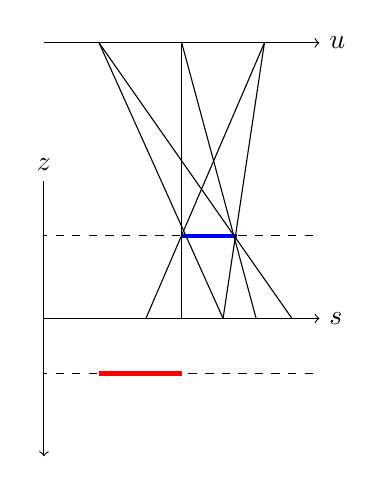
\begin{tikzpicture}[scale = 0.35]
		\draw[->] (-5, 10) -- (5, 10) node[right] {$u$};
		\draw[->] (-5, 0) -- (5, 0) node[right] {$s$};
		\draw[<-] (-5, -5) -- (-5, 5) node[above] {$z$};
	
		\begin{scope}
			\clip (-5, -5) rectangle (5, 5);
			\draw[scale = 1, smooth, domain = -10 : 10, variable = \x, black, dashed] plot ({\x}, {3});
			\draw[scale = 1, smooth, domain = -10 : 10, variable = \x, black, dashed] plot ({\x}, {-2});
		\end{scope}
		
		%\node[left] at (-5, 3) {$Z_\text{min}$};
		%\node[left] at (-5, -2) {$Z_\text{max}$};
		
		\draw[ultra thick, blue] (0, 3) -- (2, 3);
		\draw[ultra thick, red] (-3, -2) -- (0, -2);
		
		% Phantom node for alignment
		\node[right, opacity = 0] at (-5, -5) {$s$};
		
		% 1. projection
		\draw<1>[black] (-3, 10) -- (4, 0);
		\draw<1>[black] (-3, 10) -- (1.5, 0);
		
		% 2. projection
		\draw<2>[black] (0, 10) -- (2.7, 0);
		\draw<2>[black] (0, 10) -- (0, 0);
		
		% 3. projection
		\draw<3>[black] (3, 10) -- (1.5, 0);
		\draw<3>[black] (3, 10) -- (-1.3, 0);
		
	\end{tikzpicture}
\end{document}